\documentclass{beamer}

\usepackage{amssymb,amsmath}
\usepackage{graphicx}
\usepackage{url}
\usepackage{color}
\usepackage{relsize}		% For \smaller
\usepackage{url}			% For \url
\usepackage{epstopdf}	% Included EPS files automatically converted to PDF to include with pdflatex
\usepackage{pagenote}[continuous,page]

%For MindMaps
% \usepackage{tikz}%
% \usetikzlibrary{mindmap,trees,arrows}%

%%% Color Definitions %%%%%%%%%%%%%%%%%%%%%%%%%%%%%%%%%%%%%%%%%%%%%%%%%%%%%%%%%
%\definecolor{bordercol}{RGB}{40,40,40}
%\definecolor{headercol1}{RGB}{186,215,230}
%\definecolor{headercol2}{RGB}{80,80,80}
%\definecolor{headerfontcol}{RGB}{0,0,0}
%\definecolor{boxcolor}{RGB}{186,215,230}

%%% Save space in lists. Use this after the opening of the list %%%%%%%%%%%%%%%%
%\newcommand{\compresslist}{
%	\setlength{\itemsep}{1pt}
%	\setlength{\parskip}{0pt}
%	\setlength{\parsep}{0pt}
%}

%\setbeameroption{show notes on top}

% You should run 'pdflatex' TWICE, because of TOC issues.

% Rename this file.  A common temptation for first-time slide makers
% is to name it something like ``my_talk.tex'' or
% ``john_doe_talk.tex'' or even ``discrete_math_seminar_talk.tex''.
% You really won't like any of these titles the second time you give a
% talk.  Try naming your tex file something more descriptive, like
% ``riemann_hypothesis_short_proof_talk.tex''.  Even better (in case
% you recycle 99% of a talk, but still want to change a little, and
% retain copies of each), how about
% ``riemann_hypothesis_short_proof_MIT-Colloquium.2000-01-01.tex''?

\mode<presentation>
{
  % A tip: pick a theme you like first, and THEN modify the color theme, and then add math content.
  % Warsaw is the theme selected by default in Beamer's installation sample files.

  %%%%%%%%%%%%%%%%%%%%%%%%%%%% THEME
  %\usetheme{Madrid}		% No subsection
  \usetheme{AnnArbor}  % Subsection on top, no color


  %\usetheme{Antibes}
  %\usetheme{Bergen}
  %\usetheme{Berkeley}		% bem bacana - menu esquerdo
  %\usetheme{Berlin}
  %\usetheme{Boadilla}
  %\usetheme{boxes}
  %\usetheme{CambridgeUS}		% bem bacana - menu superior
  %\usetheme{Copenhagen}
  %\usetheme{Darmstadt}
  %\usetheme{default}
  %\usetheme{Dresden}
  %\usetheme{Frankfurt}
  %\usetheme{Goettingen}
  %\usetheme{Hannover}		% bem bacana - menu esquerdo
  %\usetheme{Ilmenau}
  %\usetheme{JuanLesPins}
  %\usetheme{Luebeck}
  %\usetheme{Malmoe}
  %\usetheme{Marburg}		% bem bacana - menu direito
  %\usetheme{Montpellier}
  %\usetheme{PaloAlto}		% bem bacana - menu esquerdo
  %\usetheme{Pittsburgh}
  %\usetheme{Rochester}		%bacana
  %\usetheme{Singapore}
  %\usetheme{Szeged}
  %\usetheme{Warsaw}

  %%%%%%%%%%%%%%%%%%%%%%%%%%%% COLOR THEME
  %\usecolortheme{default}		% branco, azul clarinho
  \usecolortheme{crane}		% Very yellow (ok)

  %\usecolortheme{albatross}		% azul escuro, massa
  %\usecolortheme{beetle}		% cinza, menu azul
  %\usecolortheme{dolphin}		% azul e branco, legal
  %\usecolortheme{dove}			% cinza e branco, feio
  %\usecolortheme{fly}			% todo cinza, horrível
  %\usecolortheme{lily}			% parece o default
  %\usecolortheme{orchid}		% azul e branco, ok
  %\usecolortheme{rose}			% branco e violeta-claro, bonito
  %\usecolortheme{seagull}		% cinza, feio
  %\usecolortheme{seahorse}		% nhé, meio feio
  %\usecolortheme{sidebartab}		% Azul, branco, destaque na tab, interessante
  %\usecolortheme{structure}		% bichado
  %\usecolortheme{whale}		% Azul e branco, bem bonito

  %%%%%%%%%%%%%%%%%%%%%%%%%%%% OUTER THEME
  \useoutertheme{default}
  %\useoutertheme{infolines}
  %\useoutertheme{miniframes}
  %\useoutertheme{shadow}
  %\useoutertheme{sidebar}
  %\useoutertheme{smoothbars}
  %\useoutertheme{smoothtree}
  %\useoutertheme{split}
  %\useoutertheme{tree}

  %%%%%%%%%%%%%%%%%%%%%%%%%%%% INNER THEME
  \useinnertheme{circles}
  %\useinnertheme{default}
  %\useinnertheme{inmargin}
  %\useinnertheme{rectangles}
  %\useinnertheme{rounded}

  %%%%%%%%%%%%%%%%%%%%%%%%%%%%%%%%%%%

  \setbeamercovered{invisible} % or whatever (possibly just delete it)
  % To change behavior of \uncover from graying out to totally
  % invisible, can change \setbeamercovered to invisible instead of
  % transparent. apparently there are also 'dynamic' modes that make
  % the amount of graying depend on how long it'll take until the
  % thing is uncovered.

}


% Get rid of nav bar
\beamertemplatenavigationsymbolsempty

% Use short top
%\usepackage[headheight=12pt,footheight=12pt]{beamerthemeboxes}
%\addheadboxtemplate{\color{black}}{
%\hskip0.5cm
%\color{white}
%\insertshortauthor \ \ \ \
%\insertframenumber \ \ \ \ \ \ \
%\insertsection \ \ \ \ \ \ \ \ \ \ \ \ \ \ \ \ \  \insertsubsection
%\hskip0.5cm}
%\addheadboxtemplate{\color{black}}{
%\color{white}
%\ \ \ \
%\insertsection
%}
%\addheadboxtemplate{\color{black}}{
%\color{white}
%\ \ \ \
%\insertsubsection
%}

% Insert frame number at bottom of the page.
% \usefoottemplate{\hfil\tiny{\color{black!90}\insertframenumber}}

%% makes the ppagenote command for figure references at the end.

\usepackage[english]{babel}
%qq\usepackage[latin1]{inputenc}
\usepackage{CJKutf8}
\usepackage{subfigure}

\usepackage{times}
\usepackage[T1]{fontenc}

\makepagenote
\renewcommand{\notenumintext}[1]{}
\newcommand{\ppagenote}[1]{\pagenote[Page \insertframenumber]{#1}}

\title[Programming Challenges]{GB20602 - Programming Challenges}
\author[Claus Aranha]{Claus Aranha\\{\footnotesize caranha@cs.tsukuba.ac.jp}}
\institute[U. Tsukuba]{University of Tsukuba, Department of Computer Sciences}


\title[GB21802]{GB21802 - Programming Challenges}
\subtitle[]{Week 3 - Dynamic Programming (Part I)}
\author[Claus Aranha]{Claus Aranha\\{\footnotesize caranha@cs.tsukuba.ac.jp}}
\institute{College of Information Science}
\date{2015-05-13,16\\{\tiny Last updated \today}}

\begin{document}

\section{Introduction}
\subsection{Title}
\begin{frame}
\maketitle
\end{frame}

\subsection{Notes and Warnings}

\begin{frame}
  \frametitle{Last Week Results}
  {\tiny
    \begin{columns}[T]
      \column{0.33\textwidth}
      \begin{block}{Week 0 - Simple Problems}
        Problems Solved\\
        \begin{itemize}
        \item Division Of Nlogonia: 28/28
        \item Cancer Or Scorpio: 24/27
        \item 3n+1: 25/25
        \item Request for Proposal: 19/22
        \end{itemize}

        \medskip

        Manaba Submission: 29 Students
      \end{block}
      \column{0.33\textwidth}
      \begin{block}{Week 1 - Data Structures}
        Problems Solved\\
        \begin{itemize}
          \item Jolly Jumpers: 27/27
          \item Army Buddies: 16/22
          \item Rotated Square: 18/18
          \item File Fragmentation: 5/6
          \item Contest Scoreboard: 10/11
          \item Multitasking: 5/7
          \item Jolibee Tournament: 10/10
        \end{itemize}

        \medskip

        Manaba Submission: 25 students
      \end{block}
      \column{0.33\textwidth}
      \begin{block}{Week 2 - Search Problems}
        Problems Solved (as of Thu 17:00)\\
        \begin{itemize}
        \item Division: 19/22
        \item Social Constraints: 9/9
        \item Simple Equations: 1/7
        \item Bars: 11/13
        \item Rat Attack: 9/10
        \item Little Bishops: 2/2
        \item Water Gate: 3/3
        \item Through the Desert: 4/4
        \item Dragon of Loowater: 12/13
        \item Shoemaker's Problem: 5/6
        \end{itemize}
      \end{block}
    \end{columns}
  }

  \begin{center}
    Don't Give Up!
  \end{center}
\end{frame}

\begin{frame}
  \frametitle{Special Notes}
\end{frame}

\section{Definition}
\subsection{Definition of Dynamic Programming}
\begin{frame}
  \frametitle{Dynamic Programming (DP)}

  \structure{Dynamic programming (DP)} is a more challenging, but much
  more versatile, approach for \structure{search algorithms}.

  \vfill

  \begin{block}{Basic idea of DP}
    Define a table with all unique search states of a problem, and 
    fill that table (in a top-down or bottom up fashion) until the 
    desired solution is found.
  \end{block}

  \begin{exampleblock}{Key skills needed for DP}
    \begin{itemize}
    \item Determine state space for a problem;
    \item Determine transition between spaces;
    \end{itemize}
  \end{exampleblock}
\end{frame}

\begin{frame}
  \frametitle{Uses of DP} 

  DP is most often used in \emph{optimization} or \emph{counting}
  problems.

  \vfill

  If your problem can be described as:
  \begin{itemize}
  \item Maximize this...
  \item Minimize that...
  \item Count the ways to do...
  \end{itemize}
  Then there is a very high chance that you should use DP to solve it.
\end{frame}

\subsection{Introductory Problem: Wedding}

\begin{frame}
    \frametitle{Problem Example: Wedding Shopping -- UVA 11450}

    \begin{block}{}
      Best way to understand DP is to \structure{do a lot of examples!}
    \end{block}
    
    Problem outline:
    \begin{itemize}
      \item Consider budget $M < 200$ to buy $C < 20$ classes;
      \item Each class has $K_i < 20$ items, each with different cost;
      \item \structure{Goal:} Choose one item from each class so that
        the money used is maximum; \alert{Do not go over the budget!}
    \end{itemize}

    \hfill \includegraphics[width=0.25\textwidth]{../img/weddingdress}\\
    {\tiny
    \hfill Image CC-By-2.0 by \url{https://www.flickr.com/photos/vancouver125/5634967507}}

\end{frame}

\begin{frame}
  \frametitle{Problem Example: Wedding Shopping -- UVA 11450}
  \begin{block}{Sample case 1: $C=3$}
  \begin{tabular}{|c|cccc|}
    Class & 1 & 2 & 3 & 4\\
    \hline
    0 & 6 & 4 & 8 & \\
    1 & 5 & 10 & & \\
    2 & 1 & 5 & 3 & 5\\
  \end{tabular}
  \end{block}

  \medskip

  For budget $M=20$, the answer is \alert{19}, which can be reached by buying items
  $(8+10+1)$, $(6+10+3)$ or $(4+10+5)$.

  \bigskip

  On the other hand, if the budget $M=9$, the answer is ``no
  solution'', because the minimal possible budget is \alert{10},
  reached by buying items $(4+5+1)$.
\end{frame}

\begin{frame}
  \frametitle{Problem Example: Wedding Shopping -- UVA 11450}
  \begin{block}{Sample case 1: $C=3$}
  \begin{tabular}{|c|cccc|}
    Class & 1 & 2 & 3 & 4\\
    \hline
    0 & 6 & 4 & 8 & \\
    1 & 5 & 10 & & \\
    2 & 1 & 5 & 3 & 5\\
  \end{tabular}
  \end{block}

  This looks like a search problem! Can we do a \structure{greedy search}?

  \bigskip

  One approach: For each class, choose most expensive item:\\
  $(8+10+1)$ -- It works! ... Not if $M = 12$...

  \medskip

  How about \structure{divide and conquer}?

\end{frame}

\begin{frame}
  \frametitle{Wedding Shopping (11450) -- Complete search}
  How can we enumerate the search space? (all the solutions)

  \begin{block}{Recursive Approach}
    \begin{itemize}
    \item Function \structure{shop(m,g)} discovers the best item $k$
      in class $C_g$ that can be bought with total money $m$
    \item For each $k$ in $C_g$, the value for that choice is $V_k =
      \text{cost}_k + \text{shop}(m - \text{cost}_k, g+1)$
    \item shop(m,g) returns the maximum $V_k =< m$;
    \item shop(m,$|C|$), when we pass the last item, returns 0;
    \end{itemize}

  \end{block}

  \vfill
  
  This works! ... but TLE.
\end{frame}

\begin{frame}
  \frametitle{Wedding Shopping (11450) - Complete search}
  
  \alert{Time Limit Exceeded:}

  \bigskip

  20 categories of items, with 20 items each, a complete search will
  take: $20^{20}$ operations.

  \vfill

  \alert{Problem: Too many overlapping subproblems}
  

  \begin{block}{Sample case 2: $C=4$}

    \medskip

    \begin{columns}[T]
      \column{0.4\textwidth}
      \begin{tabular}{|c|cccc|}
        Class & 1 & 2 & 3 & 4\\
        \hline
        0 & 6 & 4 & 8 & 12\\
        1 & 4 & 6 & 6 & 2\\
        2 & 1 & 5 & 1 & 5\\
        3 & 2 & 4 & 6 & 2\\
      \end{tabular}
      \column{0.4\textwidth}
      How many times \emph{shop(15,3)} is called?
      
      \bigskip

      Every time we call \emph{shop(15,3)}, the solution is the same.

    \end{columns}
  \end{block}
\end{frame}

\subsection{Dynamic Programming Approach}

\begin{frame}
  \frametitle{Wedding Shopping -- the DP approach}

  Since the problem has an \structure{overlapping subproblem}
  structure, we can think about using a DP approach.

  \bigskip

  The first step of using DP is constructing the state table.

  \smallskip

  \begin{block}{How many states do we need?}
    Since we know the unique states are \emph{(Money,Class)}, we need
    to make a table of $M x C$.

    \bigskip

    Since $0 \leq M \leq 200$ and $0 < C \leq 20$, our table will have
    \alert{$201*20=4020$ states}.
  \end{block}

  \smallskip

  Only 4020 states! This looks promising!
\end{frame}

\begin{frame}
  \frametitle{Wedding Shopping -- the DP approach}

  Now that we have our \structure{state table}, there are two
  approaches for building a DP solution:

  \bigskip

  \begin{itemize}
  \item \structure{The top-down approach}: \\Use the state table as a
    look-up table. Save the result of visited states, and do not
    re-calculate those.

    \vfill

  \item \structure{The bottom-up approach}: \\Fill the base-states of
    the table, and iteratively fill the other states transitioning
    from the base.
  \end{itemize}

\end{frame}

%%%%%%%%%%%%%%
%% Solution: Dynamic Programming
% Programming here is not "code", but a "tabular method" (table method)

%% DP us normally used when
% Program has optimal sub structure: 
%   The optimal solution to the problem contain optimal solutions to sub problems
%   - "similar" to the requirement of greedy
%   - If you can make a complete search recurrent (recursive), then you have this
% The subproblems are overlapping
%   - The number of _Distinct_ subproblems is small, but they are computed repeatedly
%   - Different from divide and conquer, in DC the sub problems are distinct
%%%%%%%%%%%%%

\begin{frame}[fragile,single-slide]
  \frametitle{Wedding Shopping -- top-down DP}

{\smaller
\begin{verbatim}
memset(table,-1,sizeof(table))  ** DP <3 memset **

shop(m,g):
   if (m < 0) return -INF
   if (g == C) return M - money
   if (table[m][g]) != -1 return table[m][g]  **NEW**
   return table[m][g] = max(shop(m-price[g][k],g+1) 
                            for every k)
\end{verbatim}  
% TODO: check if M - money is a good return value
\vfill

\begin{block}{}
  To implement top-down DP, simply add a table check to a complete
  recursive search.
\end{block}

\begin{alertblock}{}
  Make sure that your states are \alert{independent} from the
  parent. If they are not, you need to rethink your state table.
\end{alertblock}
}
\end{frame}

%%% TODO: Add how to print after the bottom up DP
%% What if you need to print the result (maybe not add this?)
% for each level, you check the lower level to see which one matches the current state
% See slide 16 for details

\begin{frame}
  \frametitle{Wedding Shopping -- bottom-up DP}
  Algorithm:
  \begin{itemize}
  \item Prepare a table with the problem states (same as top-down);
  \item Fill the table with base case values;
  \item Find the \structure{topological order} in which the table is filled;
  \item Fill the non-basic cases;
  \end{itemize}

  \vfill

  The main problem for bottom-up DP is finding the base cases and the 
  ordering between the cases. In some good cases, the ordering is 
  just a list of nested loops!
\end{frame}

\begin{frame}
  \frametitle{Wedding Shopping -- bottom-up DP}

  Example: M=10, \alert<2>{G1=(2,4)}, \alert<3>{G2=(4,6)}, \alert<4>{G3=(1,3,2,1)}

  \bigskip

  \begin{tabular}{|c||c|c|c|c|c|c|c|c|c|c|c|c|}
    \hline
    Money & 0 & 1 & 2 & 3 & 4 & 5 & 6 & 7 & 8 & 9 & 10\\
    \hline
    G0 & & & & & & & & & & & 1\\
    G1 & & & & & & & \only<2->{1} & & \only<2->{1} & & \\
    G2 & \only<3->{1} & & \only<3->{1} & & \only<3->{1} & & & & & & \\
    G3 & \only<4->{1} & \only<4->{1} & \only<4->{1} & \only<4->{1} & & & & & & & \\
    \hline
  \end{tabular}

  {\smaller
  \begin{itemize}
  \item Initial state: With 0 items, we can reach money 10;
  \item For each reachable money state in $G_i$, we can reach money
    state in $G_{i+1}$ according to the costs of the items.
  \item If any money state in $G_C$ is reachable, the problem is solvable.
  \item Solution is M - minimal reachable state;
  \end{itemize}}
\end{frame}

\begin{frame}[fragile,singleframe]
  \frametitle{Wedding Shopping -- bottom-up DP}
  M=10, cost[1] = [2,4], cost[2] =(4,6), G3=(1,3,2,1)
  \begin{tabular}{|c||c|c|c|c|c|c|c|c|c|c|c|c|}
    \hline
    Money & 0 & 1 & 2 & 3 & 4 & 5 & 6 & 7 & 8 & 9 & 10\\
    \hline
    g = 0 & & & & & & & & & & & 1\\
    g = 1 & & & & & & & 1 & & 1 & & \\
    g = 2 & 1 & & 1 & & 1 & & & & & & \\
    g = 3 & 1 & 1 & 1 & 1 & & & & & & & \\
    \hline
  \end{tabular}

  {\smaller
\begin{verbatim}
memset(table,0,sizeof(table))

table[0][10] = 1

for g in (0:G-1)
  for i in (0:M):
    if table[g][i] == 1:
       for k in C[g+1]:
          table[g+1][i-cost[k]] = 1
\end{verbatim}
  }

\end{frame}

\subsection{Considerations}

\begin{frame}
  \frametitle{DP: Top-down or Bottom-up?}
  
  \begin{block}{Top-Down}
    \structure{Pros:}\\ Easy to implement starting from a recursive
    search. Only compute states if necessary.

    \alert{Cons:}\\ Recursive calls are slower if there are many
    levels, state table memory usually can't be reduced.    
  \end{block}

  \begin{block}{Bottom-Up}
    \structure{Pros:}\\ Faser if many sub-problems are visited. Can
    sometimes save memory space by keeping only s and s+1 in memory.

    \alert{Cons:}\\ Not very intuitive. If there are X states, all
    states values will have to be checked.
  \end{block}
    


\end{frame}

\begin{frame}
  \frametitle{DP: What about the decision set?}  

  \begin{block}{}
  In the previous example, we only cared about the final value of the
  solution. What if we want to know the exact items in an optimal
  solution?
  \end{block}

  \medskip
  
  Together with the \emph{state} table, keep a second \emph{parent} table. 
  Every time you update a value on the state table, write in the parent table 
  which cell(s) was used to update that value.

  \medskip

  Pay attention to whether the problem requires you to print the first
  solution, or the last, or a solution with some particular
  properties.

  \bigskip

  Let's see some code in the next DP example.
\end{frame}
% If we need to print the decision set, we have to add a second table
% pay attention to requirements such as ortographical order, etc



\section{More Examples}
\subsection{Apple Field Example}
\begin{frame}
  \frametitle{Example 2: Apple Field -- not on UVA}

  \begin{block}{}
  {\smaller
  Farmer Tanaka is growing apples in his field. He has a robot to collect the apples, but 
  the robot can only walk east and south. If you know how many apples there are in each 
  tree of his $m * n$ field, can you calculate the path that the robot should make to collect
  most apples?}
  \end{block}
  
  \begin{center}  
    \includegraphics[width=0.5\textwidth]{../img/applefield}
  \end{center}
\end{frame}

\begin{frame}
  \frametitle{Example 2: Apple Field -- complete search}
  \begin{center}
    {\smaller One possible (non-optimal) solution}\\
    \includegraphics[width=0.5\textwidth]{../img/applefield-solution}
  \end{center}

  For every square, the robot can choose to go right (east) or down
  (south). How many possible paths exist?

  \bigskip

  And how many overlapping solutions are there?
\end{frame}

\begin{frame}
  \frametitle{Example 2: Apple Field -- overlapping solutions}
  \begin{center}
    {\smaller One possible (non-optimal) solution}\\
    \includegraphics[width=0.5\textwidth]{../img/applefield-solution}
  \end{center}

  If the robot reached position (x,y) with k apples, it does not
  matter how it did it. So the path from (x,y) to the goal is independent from 
  the parent path.

  This smells like DP! Let's solve it with a bottom up approach.
\end{frame}

\begin{frame}
  \frametitle{Example 2: Apple Field -- Bottom up DP}

  {\small
  \begin{itemize}
  \item \structure{tables:} We want to maximize the number of apples
    at the goal. Let's try a m*n position table. At each cell, we want
    to store the maximum number of apples achievable at that cell.

    \medskip

    We also want a second table, \emph{path}, which will store the path
    used.

    \vfill
    
  \item \structure{initial condition:} We can fill the top row (x,1) of the 
    table with the sum of apples from 1 to x. And we can fill the Left column
    with the sum of apples from 1 to y.
    
    \medskip

    Alternatively, we can add an additional dummy ``-1'' column/line
    and fill it with zeros.

    \vfill

  \item \structure{transition:} For each cell x,y, max(x,y) is either 
    max(x-1,y) + apple(x,y) or max(x,y-1) + apple(x,y)
  \end{itemize}}  
\end{frame}

\begin{frame}[fragile,singleslide]
  \frametitle{Example 2: Apple Field -- Let's see some code}
  {\smaller
\begin{verbatim}
// Assume apple[0,] and apple[,0] are all zeroes.
int apple[m][n]// Input.
int sum[m][n]// DP table, set to 0 using memset
int parent[m][n][2]// Path table, set to 0 using memset

for i in (1:m):
  for j in (1:n):
    sum[m][n] = apple[m][n] + max(sum[m][n-1],sum[m-1][n])
    if (sum[m][n-1] > sum[m-1][n]):
       parent[m][n][0] = m, parent[m][n][1] = n-1
    else:
       parent[m][n][0] = m-1, parent[m][n][1] = n
\end{verbatim}
  }
\end{frame}

\subsection{Flight Planner}
%%%%%%%%%%%%%
%% Example 2 -- UVA 10337 Flight Planner
% 1 Mile Altitude and 1(x100) miles distance
% wind speed map
% fuel cost: Climb +60, hold +30, sink +20 - windspeed wsp[alt][dis]
% Compute min fuel cost from (0,0) to (0,X=4)

%% First guess: Complete search/Backtracking finding path with minimal fuel cost
% Recurrence: minimum of current + climb/Hold/Dive
% Problem: 1000 distance columns: 3^1000 states to search!
% However, there are MANY overlapps: at any column/height, former path does not matter.

%% DP solution
% TOP down: create a 2D table and store computation value of subproblems as they are seen.
% Bottom-up: Start at 0 fuel used. Calculate next column based on where current column can reach
%            Bottom up hint: We just need to store two columns at a time (if only final result is desired)

\subsection{classical DPs}


%%%%%%%%%%%%%%%%%%%%%%%%%%%%%%%
%% Discussion on Classical DPs
% Max sum (1-D) -- Kadane's algorithm
% Longest Increasing Subsequence O(nlogk)
% 0-1 knapsack/subset sum
% Coin change (textbook)
% Travelling Salesman Problem (bitmask again)

%% Max Sum (1D)
% Given an array with positive and negative numbers, find a contiguous *sub array* with
% the max sum.
% example: 1,-2,6,3,2,-12,-6,7,1
% answer is: 6,3,2 -- can we do this in On^3? n^2? n?

%% Longest Increasing Subsequence
% Find the LIS in an array A -- subsequence does not need to be contiguous
% Example: -7, 10, 9, 2, 3, 8, 8, 1: How to do it in n^2? How to do it in nLogK?
% Answer above is -7,2,3,8

%% 0/1 Knapsack/subset sum
% Items have weight and price
% n item, S backpack size: can we do it in O(nS)

%% Travelling Salesman Problem (TSP)
% State: tsp(pos,bitmask)
% Transition: 
%   Each visited city is a bit in the bitmask
%   - if every city has been visited: tsp(pos, 2^n -1) = dist[pos][0] (back to the start with 0 cities)
%   - Else, try visiting unvisited cities one by one
%   - tsp(pos,bitmask) = min (dist[pos][nxt] + tsp(nxt,bitmask|1<<nt))) for every nxt != pos, 
%                                                                           and nxt not visited
%                                                                           bitmask & 1<<nxt == 0

\section{Conclusion}
\subsection{Conclusion}
\begin{frame}
   \frametitle{Summary} 

   Dynamic Programming is a \structure{smart way to do complete
     search}, when a large part of the search space is overlapping.

   \begin{itemize}
   \item \alert{Top-down DP}: recursive complete search with memoization;
   \item \alert{Bottom-up DP}: state table with iterative completion recurrency;
   \end{itemize}

   \vfill

   \begin{block}{Next Class}
     \begin{itemize}
     \item DP on non-classical problems
     \item Relationship between DP and DAG
     \item Other ``cool'' DP techniques.
     \end{itemize}
   \end{block}
\end{frame}

\begin{frame}
   \frametitle{Read more about DP}
   \begin{itemize}
      \item \url{http://people.csail.mit.edu/bdean/6.046/dp/}
      \item \url{http://community.topcoder.com/tc?module=Static&d1=tutorials&d2=dynProg}
   \end{itemize}
\end{frame}

\subsection{This Week's Problems}
\begin{frame}
   \frametitle{This Week's Problems}
   \begin{itemize}
   \item Jill Rides Again
   \item Maximum Sum on a Torus
   \item Strategic Defense Initiative
   \item Is bigger smarter?
   \item Ferry Loading
   \item Unidirectional TSP
   \item Flight Planner
   \item e-Coins
   \end{itemize}
\end{frame}


\section{Extra}
\subsection{Extra}
%% TODO: Add another call for action regarding programming contests? -- DP is a big part of progcon.

% DP is a very important program paradigm in programming contests
\end{document}



